%%%%%%%%%%%%%%%%%%%%%%%%%%%%%%%%%%%%%%%%%%
\section{Part 2 - Exercise 0 - p40}
%%%%%%%%%%%%%%%%%%%%%%%%%%%%%%%%%%%%%%%%%%
%
\begin{equation*}
    \min_{\bs x \in \Rbb^n}~\norm{\bs{Ax}-\bs b}{2}^2
    + \underbrace{\frac{\lambda_1}{2} \norm{\bs x}{2}^2 
    + \lambda 2 \norm{\bs x}{1}}_{\text{elastic net}},
\end{equation*}
%
where $\bs A \in \Rbb^{m\times n}$, $\bs \in \Rbb^m$ and 
$\lambda_1, \lambda_2>0$.
%
Choosing $f(\bs x) = \norm{\bs{Ax}-\bs b}{2}^2 
+ \frac{\lambda_1}{2} \norm{\bs x}{2}^2$ as the $\sigma$-strongly 
convex and differentiable part and 
$g(\bs x) = \lambda_2 \norm{\bs x}{1}$ as the closed 
convex but non differentiable part, one has 
$\nabla f(\bs x) = \bs A^\top (\bs{Ax}-\bs b) + \lambda_1 
\bs{Ix}$ and $\prox_{\lambda g}(\bs x) = 
\soft{\lambda_2}(\bs x)$.
%
\begin{itemize}
    \item (\emph{Proximal Gradient})
    \begin{align*}
    \begin{split}
        \bs x^{k+1} &= \prox_{\tinv L g}(\bs x^k - \tinv L 
        \nabla f(\bs x^k)) \\
        &= \soft{\frac{\lambda_2}{L}} \left( \bs x^k 
        - \tinv L (\ATA + \lambda_1 \bs I) 
        \bs x^k + \tinv L \bs A^\top\bs b
        \right),
    \end{split}
    \end{align*}
    %
    with $L = \norm{\ATA + \lambda_1 \bs I}{}
    = \lambda_{\max} (\ATA) + \lambda_1 = \norm{\bs A}{2}^2
    + \lambda_1$.
    \item (\emph{FISTA})
    \begin{align*}
    \begin{split}
    \left\{
    \begin{array}{lll}
        \bs x^{k+1} &= \soft{\frac{\lambda_2}{L}} 
        \left( \bs y^k - \tinv L (\ATA + \lambda_1 \bs I) 
        \bs y^k + \tinv L \bs A^\top\bs b \right) \\
        t_{k+1} &= \frac{1+\sqrt{1+4t_k^2}}{2} \\
        \bs y^{k+1} &= \bs x^{k+1} + \left( 
        \frac{t_k-1}{t_{k+1}} \right) (\bs x^{k+1}- \bs x^k)
    \end{array}
    \right.
    \end{split}
    \end{align*}
    \item (\emph{V-FISTA})
    \begin{align*}
    \begin{split}
    \left\{
    \begin{array}{ll}
        \bs x^{k+1} &= \soft{\frac{\lambda_2}{L}} 
        \left( \bs y^k - \tinv L (\ATA + \lambda_1 \bs I) 
        \bs y^k + \tinv L \bs A^\top\bs b \right) \\
        \bs y^{k+1} &= \bs x^{k+1} + \left( 
        \frac{\sqrt\kappa-1}{\sqrt\kappa+1} \right) 
        (\bs x^{k+1}- \bs x^k),
    \end{array}
    \right.
    \end{split}
    \end{align*}
    %
    with $\kappa=L/\sigma$, and $\sigma=1$.
\end{itemize}
%
Now, if one chooses $f(\bs x) = \norm{\bs{Ax}-\bs b}{2}^2$ 
as the differentiable (but not strongly convex) part and 
$\alpha g(\bs x) = \frac{\alpha\lambda_1}{2} \norm{\bs x}{2}^2 
+ \alpha\lambda_2 \norm{\bs x}{1}$ as the closed 
convex but non differentiable part, one has 
$\nabla f(\bs x) = \bs A^\top (\bs{Ax}-\bs b)$ and, 
by identification with $g'(\bs x) + \frac{c}{2} 
\norm{\bs x}{2}^2 + \scp{\bs a}{\bs x} + \gamma$ with 
$g'(\bs x) = \alpha\lambda_2 \norm{\bs x}{1}, 
c=\alpha\lambda_1, \bs a=\bs 0, \gamma=0$, 
$\prox_{\alpha g}(\bs x) = 
\prox_{\frac{\alpha}{\alpha\lambda_1+1} \lambda_2 
\norm{\cdot}{1}} (\frac{\bs x}{\alpha\lambda_1+1}) = 
\soft{\frac{\alpha\lambda_2}{\alpha\lambda_1+1}} 
(\frac{\bs x}{\alpha\lambda_1+1})$.
%
\begin{itemize}
    \item (\emph{V-FISTA2})
    \begin{align*}
    \begin{split}
        \left\{
        \begin{array}{ll}
            \bs x^{k+1} &= \soft{\frac{\lambda_2/L_2}{
            \lambda_1/L_2 + 1}} 
            \left( \bs y^k - \tinv{L_2} (\ATA) 
            \bs y^k + \tinv L \bs A^\top\bs b \right) \\
            \bs y^{k+1} &= \bs x^{k+1} + \left( 
            \frac{\sqrt{\kappa_2}-1}{\sqrt{\kappa_2}+1} 
            \right) (\bs x^{k+1}- \bs x^k),
        \end{array}
        \right.
    \end{split}
    \end{align*}
    %
    with $L_2=\norm{\bs A}{2}^2$, $\kappa_2=L_2/\sigma$, 
    and $\sigma=1$.
\end{itemize}
%
One notices the only difference between \emph{V-FISTA} and 
\emph{V-FISTA2} occurs in the second line, with $\kappa_2
\neq \kappa$.
%
\begin{figure}[H]
    \centering
    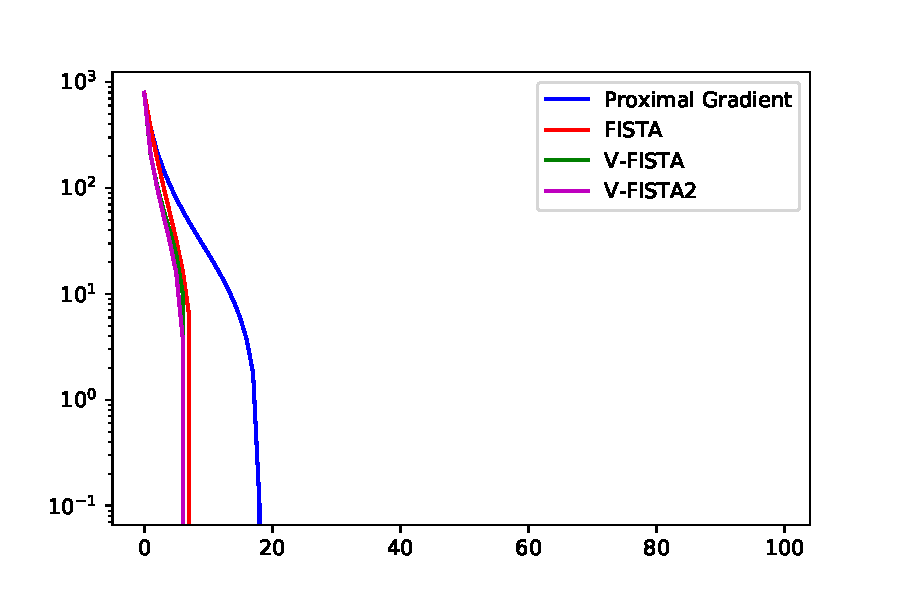
\includegraphics[width=14cm]{images/part2_ex0.pdf}
    \caption{$F(\bs x^k)-F_{\text{opt}}$ in log-scale along the 
  y-axis for the first 100 iterations of each of the methods 
  with all-zeros vectors and a constant stepsize. }
  \label{fig: ex0}
\end{figure}
%
As can be observed in Fig.~\ref{fig: ex0}, the V-FISTA 
methods worked the best, with a slight improvement in 
V-FISTA which does not follow the theory.
The four first elements are:
\begin{itemize}
    \item (-0.40403765  0.18475212  0.97264407 -0.99645397)
    \item (-0.43969331  0.01974521  1.42280231 -0.87819581)
    \item (-0.4319773   0.02881602  1.43373682 -0.9066518 )
    \item (-0.43207117  0.02954933  1.43438138 -0.9058778 )
    \item (-0.43210892  0.02959727  1.43437048 -0.9058291 )
\end{itemize}
%
for the Ground truth, and the four methods, PG, FISTA,
V-FISTA, V-FISTA2, respectively.